\section{Overview}
\label{sec:overview}

Overview of Approach (a nice and accessible ``English'' description of
your approach). Don't forget a niche high-level figure. Our sample
high-level figure is shown in Figure~\ref{fig:overview}.

There is sometimes a background section before the overview section. In
general, you want to try to get your high level figure somewhere between
pages 2 and 4. It is generally bad to have a figure on the first page
(but was unavoidable in this sample).

% You may need to move this \begin{figure} ... \end{figure} block around
% in the document to place it in a logical spot in the paper. In
% general, get the figure on the same page as the prose that refers to
% it.
\begin{figure}[t]
  \centering
  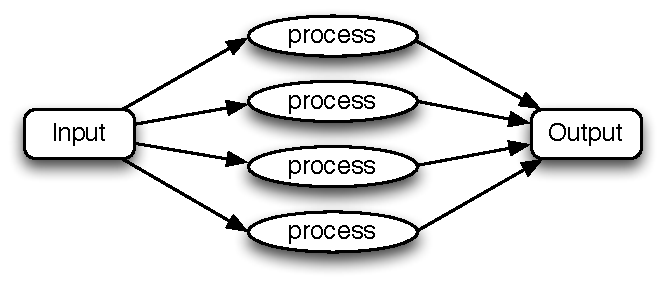
\includegraphics[width=3in]{figs/overview}
  \caption{A high-level architecture of our approach}
  \label{fig:overview}
\end{figure}
